\documentclass{amsart}

\input{../preamble_general.tex}

\author{Jalen Chrysos}
\title{Hamiltonian Paths and Cycles (with solutions)}

\begin{document}
	
	\maketitle 
	
	A \textit{Hamiltonian Path} is a path which includes every vertex exactly once. Similarly, a \textit{Hamiltonian Cycle} is a cycle which includes every vertex exactly once. In general, it is not easy to tell whether a graph has a Hamiltonian path/cycle, unlike with Eulerian paths and cycles, where one can determine the existence of a path by checking vertices' degrees.\\
	
	\noindent \textbf{Problem 1}: Let $G_{a,b}$ be the graph consisting of $ab$ vertices arranged in an $a\times b$ grid, with adjacent vertices connected by an edge. 
	\begin{enumerate}[(i)]
		\item For which $a,b$ does $G_{a,b}$ have a Hamiltonian path?
		\item For which $a,b$ does $G_{a,b}$ have a Hamiltonian cycle?\\
	\end{enumerate}
	
	\textbf{Solution}: \\
	
	(i): There is a Hamiltonian path for every $a,b$. Consider this snaking shape:
	
	\begin{figure}[h]
		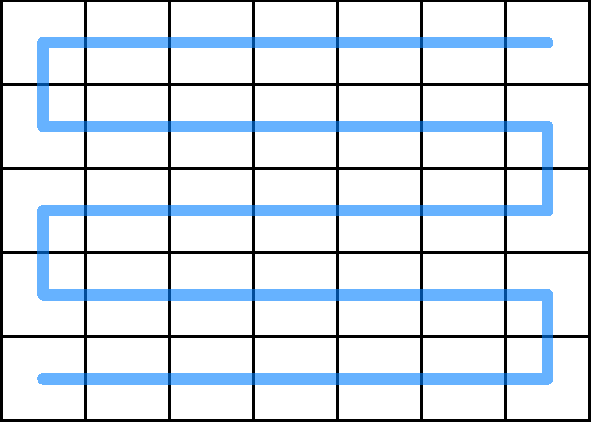
\includegraphics[width=6cm]{./Asymptote_Figs/Hamiltonian1.pdf}
	\end{figure}
	
	(ii): There is a Hamiltonian cycle if and only if one of $a,b$ is even. If for example $a$ is even, then one can use the following general pattern:
	
	\begin{figure}[h]
		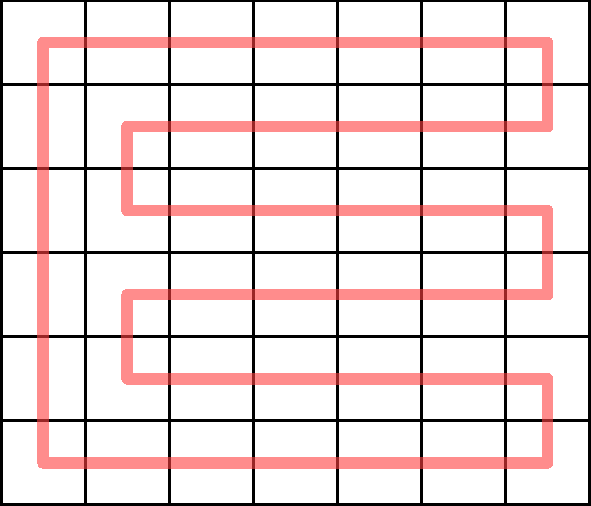
\includegraphics[width=6cm]{./Asymptote_Figs/Hamiltonian2.pdf}
	\end{figure}
	
	On the other hand, if $a$ and $b$ are both odd, then there is no cycle: color the grid with a checkerboard pattern. One can see that every path alternates between black and white squares. Because $ab$ is odd, there are more squares of one color than the other. Thus every Hamiltonian path must start and end on the more common color, so no Hamiltonian path can be joined to make a cycle.
	
	\begin{figure}[h]
		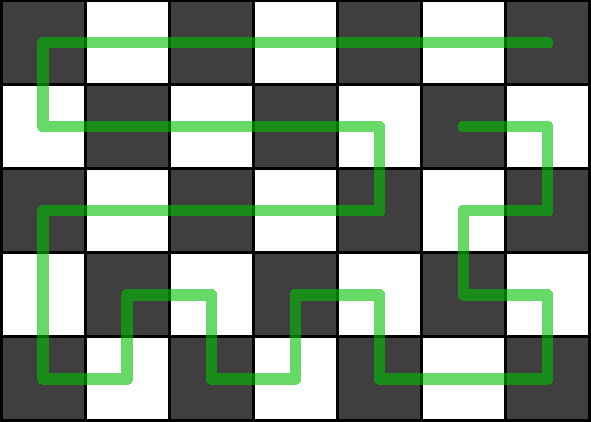
\includegraphics[width=6cm]{./Asymptote_Figs/Hamiltonian3.pdf}
	\end{figure}
	%	\noindent \textbf{Problem 2}: Which platonic solid graphs have a Hamiltonian path / cycle?\\
	%	
	%	$$\textbf{illustration of the platonic solids}$$
	
	\noindent \textbf{Problem 2}: Show that if $G$ has a Hamiltonian path, then any induced subgraph $G^*$ obtained by deleting $k$ vertices of $G$ must have at most $k+1$ connected components.\\
	
	\textbf{Solution}: Removing $k$ vertices from a path yields at most $k+1$ segments of the path. Since edges in the path are also edges of $G$, these $k+1$ segments are connected in $G$ and hence $G^*$, so there can be at most $k+1$ connected components in $G^*$.\\
	
	\noindent \textbf{Problem 3}: An (open) \textit{knight's tour} is a sequence of knight moves on a rectangular grid such that the knight visits every square exactly once (the start and end squares count as visited). Show that that a knight's tour is impossible on the following board sizes:
	\begin{enumerate}[(i)]
		\item $3\times 3$
		\item $4\times 4$
		\item $3\times 6$\\
	\end{enumerate}
	
	\textbf{Solution}: These problems can be solved efficiently by using problem 2. See the figure below:
	
	\begin{figure}[h]
		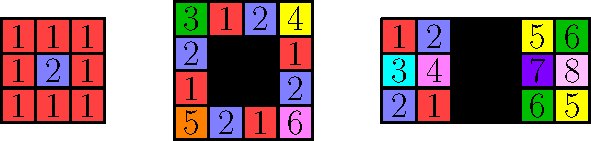
\includegraphics[width=12cm]{./Asymptote_Figs/KnightsTour.pdf}
	\end{figure}
	
	In the first case, removing $0$ vertices leaves $2$ connected components; in the second, removing $4$ leaves $6$; and in the third, removing $6$ leaves 8. By problem 2, none of these graphs can have a Hamiltonian path.\\
	
	\newpage 
	
	\noindent \textbf{Problem 4}: Find a \textit{connected} 3-regular graph (i.e. graph whose vertices all have degree 3) without any Hamiltonian path.\\
	
	\textbf{Solution}: We would like to construct a graph $G$ with a single vertex $v$ such that, if removed, would split $G$ into 3 connected components. Then by problem 2, $G$ has no Hamiltonian path. An example of such a graph is below:
	
	\begin{figure}[h]
		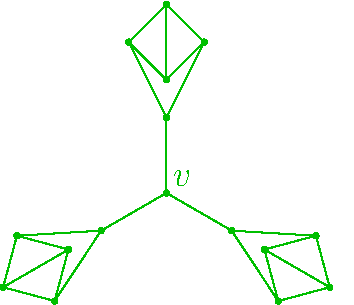
\includegraphics[width=6cm]{./Asymptote_Figs/3Regular.pdf}
	\end{figure}
	
	\noindent \textbf{Problem 5}: Let $G_n$ be the $n$-dimensional cube graph; that is, $G_n$ has $2^n$ vertices corresponding to binary strings $(0,1,1,0,\dots)$ of length $n$, and two strings have an edge between them if and only if they differ in exactly one place (e.g. $(0,1,1)\sim (1,1,1)$ but $(0,1,1)\not\sim (1,0,1)$). Show that $G_n$ has a Hamiltonian cycle for all $n\geq 2$.\\
	
	\textbf{Solution}: This can be done by induction on $n$: $G_2$ is a square, so it clearly has a Hamiltonian cycle. Now, assuming $G_n$ has a Hamiltonian cycle, we will construct one for $G_{n+1}$: $G_{n+1}$ can be viewed as two copies of $G_n,G_n'$, joined only by edges between each vertex in $G_n$ and its twin in $G_n'$. See below: each copy of $G_n$ is in red, and the edges connecting them are in blue.
	
	\begin{figure}[h]
		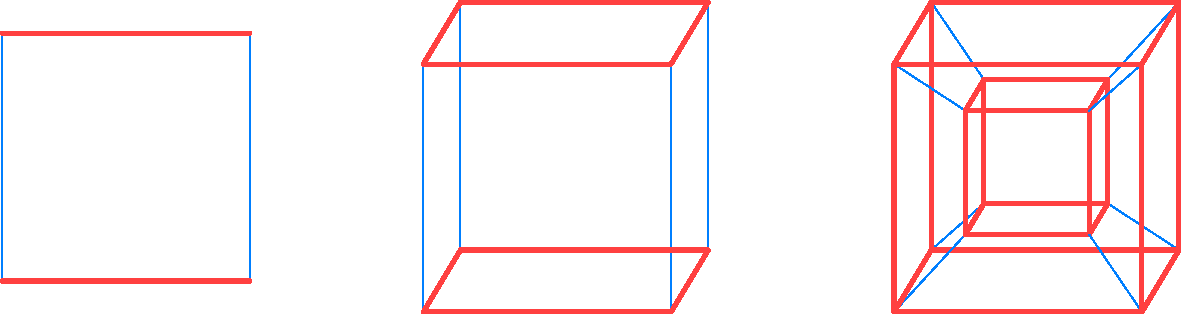
\includegraphics[width=15cm]{./Asymptote_Figs/Cubes1.pdf}
	\end{figure}
	
	Thus, taking a Hamiltonian path $P$ in $G_n$, we can also add the corresponding path $P'$ in $G_n'$ and connect the ends to create a Hamiltonian cycle:
	
	\begin{figure}[h]
		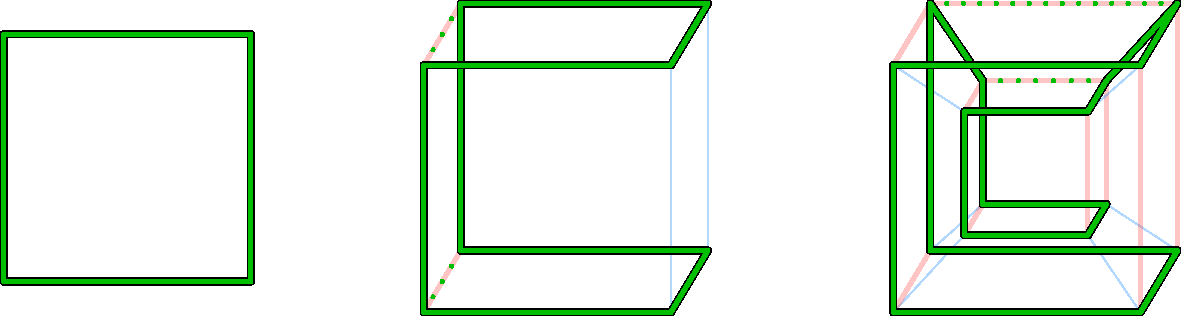
\includegraphics[width=15cm]{./Asymptote_Figs/Cubes2.pdf}
	\end{figure}
	
	The dotted green lines denote the edges that are removed from the Hamiltonian cycles so that they can be connected.
	
	\newpage 
	
	\noindent \textbf{Problem 6} ($\star$): Let $G$ be a graph on $n\geq 3$ vertices.
	\begin{enumerate}[(i)]
		\item Show that if $G$ has no Hamiltonian cycle, and $x,y$ are vertices such that $x\not\sim y$ and
		$$
		\deg(x)+\deg(y)\geq n,
		$$
		then the graph $G^+$ obtained by adding an edge $x\sim y$ also has no Hamiltonian cycle\footnote{If one takes a graph $G$ and repeatedly adds edges between any two vertices $x,y$ for which $\deg(x)+\deg(y)\geq n$, the resulting graph is called the \textit{closure} of $G$. This problem shows that $G$ has a Hamiltonian cycle if and only if its closure does.}.
		\item (Ore's Theorem): Show that if $\deg(x)+\deg(y)\geq n$ for all $x\not\sim y$, $G$ has a Hamiltonian cycle.
		\item (P\'osa's Theorem): Show that if $G$ has no Hamiltonian cycle, then for some $1\leq d<n/2$, there are at least $d$ vertices with degree $\leq d$. (\textit{Hint: It suffices to show this for the closure of $G$. Consider the set of non-neighbors of a suitable vertex $x$}).
		\item Suppose that $n=9$ and $G$ has score $(2,3,4,5,\ast,\ast,\ast,\ast,\ast)$, where each $\ast$ is some number $\geq 5$. Show that $G$ has a Hamiltonian cycle.\\
	\end{enumerate}
	
	\textbf{Solution}:\\
	
	(i): If $G^+$ has a Hamiltonian cycle, then it must be that there is a Hamiltonian path in $G$ whose endpoints are $x$ and $y$. Let this path be
	$$
	x = v_0 \sim v_1 \sim \cdots \sim v_n = y.
	$$
	Because $\deg(x)+\deg(y)\geq n$, by pigeonhole principle there must be some $x\sim v_k$ for which $y\sim v_{k+1}$. But then $G$ \textit{does} have a Hamiltonian cycle:
	$$
	x \sim v_1 \sim \cdots \sim v_k \sim y \sim v_{n-1} \sim v_{n-2} \sim \cdots \sim v_{k+1} \sim x,
	$$
	which is a contradiction. Thus, $G^+$ has no Hamiltonian cycle.\\
	
	(ii): If $\deg(x)+\deg(y)\geq n$ for all $x\not\sim y$, then by (i) we can add in edges between each $x$ and $y$ without affecting whether or not $G$ has a Hamiltonian cycle, but this results in a complete graph, which clearly has a Hamiltonian cycle, so $G$ must have had one to begin with.\\
	
	(iii): Suppose $G$ has no Hamiltonian cycle, and let $\overline{G}$ be the closure of $G$. By part (i), $\overline{G}$ has no Hamiltonian cycle. I claim that the result is true of $\overline{G}$, which implies that it is true for $G$ as well, because any vertex with degree $\leq d$ in $\overline{G}$ also has degree $\leq d$ in $G$.\\
	
	If $\overline{G}$ has $< n/2$ vertices of degree $\geq n/2$ then the claimed result holds for $d=\lceil n/2 - 1 \rceil$. On the other hand, if all the vertices of degree $\geq n/2$ (of which there are at least $n/2$) have degree $n-1$, then all vertices must have degree $\geq n/2$, but this forces $\overline{G}$ to have a Hamiltonian cycle by (ii).\\
	
	Thus, we reduce to the case in which there is at least one vertex $x$ of degree $n/2 \leq p < n-1$. $x$ has $d:= n-p-1$ non-neighbors (and note $1\leq d < n/2$). Each of its non-neighbors has degree less than $n-p$, because $\overline{G}$ is closed. Thus, the non-neighbors of $x$ have degree at most $d$, and there are $d$ of them.\\
	
	(iv): The constraint on the score of $G$ shows that there is exactly 1 vertex of degree $\leq 2$, 2 vertices of degree $\leq 3$, and $3$ vertices of degree $\leq 4$. By (iii), $G$ must have a Hamiltonian path.
	
	
	
	
\end{document}